\documentclass{beamer}

\usecolortheme[light]{solarized}

\beamertemplatenavigationsymbolsempty


\usepackage{booktabs}
\usepackage{graphicx}
\usepackage{hyperref}
\usepackage{minted}
\usepackage{moresize}
\usepackage{centernot}
\usepackage{standalone}
\usepackage{tcolorbox}
\usepackage{tikz}
\usepackage[normalem]{ulem}
\usepackage{xpatch}
\usepackage{fix-cm}
\usepackage{siunitx}

\usepackage{bibentry}
\usepackage{biblatex}
\bibliography{../refs}

\newtheorem{proposition}{Proposition}

\xpatchcmd{\sout}
  {\bgroup}
    {\bgroup\def\ULthickness{2pt}}
      {}{}

\usetikzlibrary{calc, patterns}
\usetikzlibrary{arrows}
\usetikzlibrary{decorations.markings}
\usetikzlibrary{decorations.text}
\usetikzlibrary{arrows.meta}
\usetikzlibrary{shapes.geometric,positioning}

\definecolor{traitor}{HTML}{b2182b}
\definecolor{faithful}{HTML}{2166ac}
\definecolor{dead}{HTML}{cccccc}
\definecolor{accent}{HTML}{1b7837}
\definecolor{warn}{HTML}{e08214}
\definecolor{panelbg}{HTML}{fafafa}
% Colorblind-safe social colours (Okabe-Ito palette).
\definecolor{socialmastodon}{HTML}{0072B2}
\definecolor{socialbluesky}{HTML}{009E73}
\definecolor{sociallinkedin}{HTML}{D55E00}

\begin{document}

    \begin{frame}
        \begin{center}
            \large
            The Vote-Left Equilibrium: A Deterministic Coordination Strategy for the Faithful in The Traitors

               \vfill
               \Large
               Vince Knight, Cardiff
        \end{center}
    \end{frame}

\begin{frame}[fragile]
        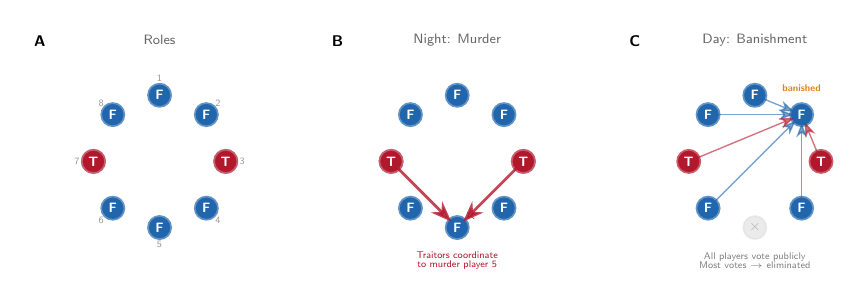
\begin{tikzpicture}[
                >=Stealth,
                font=\sffamily,
                player/.style={circle, minimum size=12pt, inner sep=0pt, line width=0.6pt,
                font=\sffamily\scriptsize\bfseries, text=white},
                fnode/.style={player, fill=faithful, draw=faithful!70},
                tnode/.style={player, fill=traitor, draw=traitor!70},
                dnode/.style={player, fill=dead, draw=dead!80, opacity=0.4,
                font=\sffamily\scriptsize\bfseries, text=black!60},
                votearrow/.style={->, line width=0.5pt, opacity=0.6},
                killarrow/.style={->, line width=1.0pt, traitor, opacity=0.8},
                panellabel/.style={font=\sffamily\footnotesize\bfseries, anchor=north west},
                caption/.style={font=\sffamily\scriptsize, text=black!60, align=center},
                scale=.7,
                transform shape,
                ]

                % ── Layout: 2 rows x 3 cols, each panel ~4.2cm wide ──
                \def\pw{4.8}   % panel width
                \def\ph{4.2}   % panel height
                \def\gap{0.6}  % gap between panels
                \def\R{1.2}    % circle radius for players

                % Panel origins (bottom-left of each)
                \coordinate (P1) at (0, \ph+\gap);
                \coordinate (P2) at (\pw+\gap, \ph+\gap);
                \coordinate (P3) at (2*\pw+2*\gap, \ph+\gap);
                \coordinate (P4) at (0, 0);
                \coordinate (P5) at (\pw+\gap, 0);
                \coordinate (P6) at (2*\pw+2*\gap, 0);

                % ── Helper: draw 8 players in a circle ──
                % Args: center, prefix, traitor list (1-indexed)
                \newcommand{\drawplayers}[3]{
                    % #1 = center, #2 = prefix, #3 = comma-separated traitor positions
                    \foreach \i in {1,...,8} {
                        \pgfmathsetmacro{\angle}{90 - (\i-1)*45}
                        \coordinate (#2-\i) at ($(#1) + (\angle:\R)$);
                    }
                    % Draw faithful first (F label), then traitors on top (T label)
                    \foreach \i in {1,...,8} {
                        \node[fnode] at (#2-\i) {F};
                    }
                    \foreach \t in {#3} {
                        \node[tnode] at (#2-\t) {T};
                    }
                    }

                    % ══════════════════════════════════════════════════════════════
                    % TOP ROW: Game phases
                    % ══════════════════════════════════════════════════════════════

                    % ── Panel A: Roles ──
                    \begin{scope}[shift=(P1)]
                        %\draw[draw=black!20, fill=white, rounded corners=3pt] (-0.3, -0.3) rectangle (\pw+0.3, \ph+0.3);
                        \node[panellabel] at (0, \ph+0.15) {A};
                        \node[caption] at (\pw/2, \ph-0.05) {Roles};

                        \pgfmathsetmacro{\cx}{\pw/2}
                        \pgfmathsetmacro{\cy}{\ph/2 - 0.15}
                        \coordinate (CA) at (\cx, \cy);
                        \drawplayers{CA}{a}{3,7}

                        % % Legend
                        % \node[fnode, minimum size=10pt] at (3.35, 0.6) {F};
                        % \node[font=\sffamily\tiny, text=faithful, anchor=west] at (3.55, 0.6) {Faithful};
                        % \node[tnode, minimum size=10pt] at (3.35, 0.25) {T};
                        % \node[font=\sffamily\tiny, text=traitor, anchor=west] at (3.55, 0.25) {Traitor};

                        % Player numbers
                        \foreach \i in {1,...,8} {
                            \pgfmathsetmacro{\angle}{90 - (\i-1)*45}
                            \node[font=\sffamily\tiny, text=black!40] at ($(CA) + (\angle:\R+0.3)$) {\i};
                        }
                    \end{scope}

                    \pause
                    % ── Panel B: Night (Murder) ──
                    \begin{scope}[shift=(P2)]
                        %\draw[draw=black!20, fill=white, rounded corners=3pt] (-0.3, -0.3) rectangle (\pw+0.3, \ph+0.3);
                        \node[panellabel] at (0, \ph+0.15) {B};
                        \node[caption] at (\pw/2, \ph-0.05) {Night: Murder};

                        \pgfmathsetmacro{\cx}{\pw/2}
                        \pgfmathsetmacro{\cy}{\ph/2 - 0.15}
                        \coordinate (CB) at (\cx, \cy);
                        \drawplayers{CB}{b}{3,7}

                        % Murder arrow: traitors 3 and 7 target faithful 5
                        \draw[killarrow, shorten >=3pt, shorten <=3pt] (b-3) -- (b-5);
                        \draw[killarrow, shorten >=3pt, shorten <=3pt] (b-7) -- (b-5);

                        % X on victim
                        \node[font=\sffamily\scriptsize\bfseries, text=traitor] at ($(b-5)+(0.25, 0.2)$) {$\times$};

                        % Annotation
                        \node[font=\sffamily\tiny, text=traitor, align=center] at (\pw/2, 0.15) {Traitors coordinate\\[-1pt]to murder player 5};
                    \end{scope}

                    \pause
                    % ── Panel C: Day (Banishment) ──
                    \begin{scope}[shift=(P3)]
                        %\draw[draw=black!20, fill=white, rounded corners=3pt] (-0.3, -0.3) rectangle (\pw+0.3, \ph+0.3);
                        \node[panellabel] at (0, \ph+0.15) {C};
                        \node[caption] at (\pw/2, \ph-0.05) {Day: Banishment};

                        \pgfmathsetmacro{\cx}{\pw/2}
                        \pgfmathsetmacro{\cy}{\ph/2 - 0.15}
                        \coordinate (CC) at (\cx, \cy);

                        % Player 5 is dead
                        \foreach \i in {1,...,8} {
                            \pgfmathsetmacro{\angle}{90 - (\i-1)*45}
                            \coordinate (c-\i) at ($(CC) + (\angle:\R)$);
                        }
                        \foreach \i in {1,2,4,6,8} {
                            \node[fnode] at (c-\i) {F};
                        }
                        \node[tnode] at (c-3) {T};
                        \node[tnode] at (c-7) {T};
                        \node[dnode] at (c-5) {$\times$};

                        % Show some votes converging on player 2 (banished)
                        \foreach \src in {1,4,6,8} {
                            \draw[votearrow, faithful, shorten >=3pt, shorten <=3pt] (c-\src) -- (c-2);
                        }
                        \draw[votearrow, traitor, shorten >=3pt, shorten <=3pt] (c-3) -- (c-2);
                        \draw[votearrow, traitor, shorten >=3pt, shorten <=3pt] (c-7) -- (c-2);

                        % Banished marker
                        \node[font=\sffamily\tiny\bfseries, text=warn, anchor=south] at ($(c-2)+(0, 0.3)$) {banished};

                        \node[font=\sffamily\tiny, text=black!50, align=center] at (\pw/2, 0.15) {All players vote publicly\\[-1pt]Most votes $\to$ eliminated};
                    \end{scope}

                \end{tikzpicture}
            \end{frame}

    \begin{frame}
        \begin{center}
            
\includegraphics[width=.9\textwidth]{./assets/claudia.jpg}
        \end{center}
    \end{frame}

    \begin{frame}
        \begin{center}
            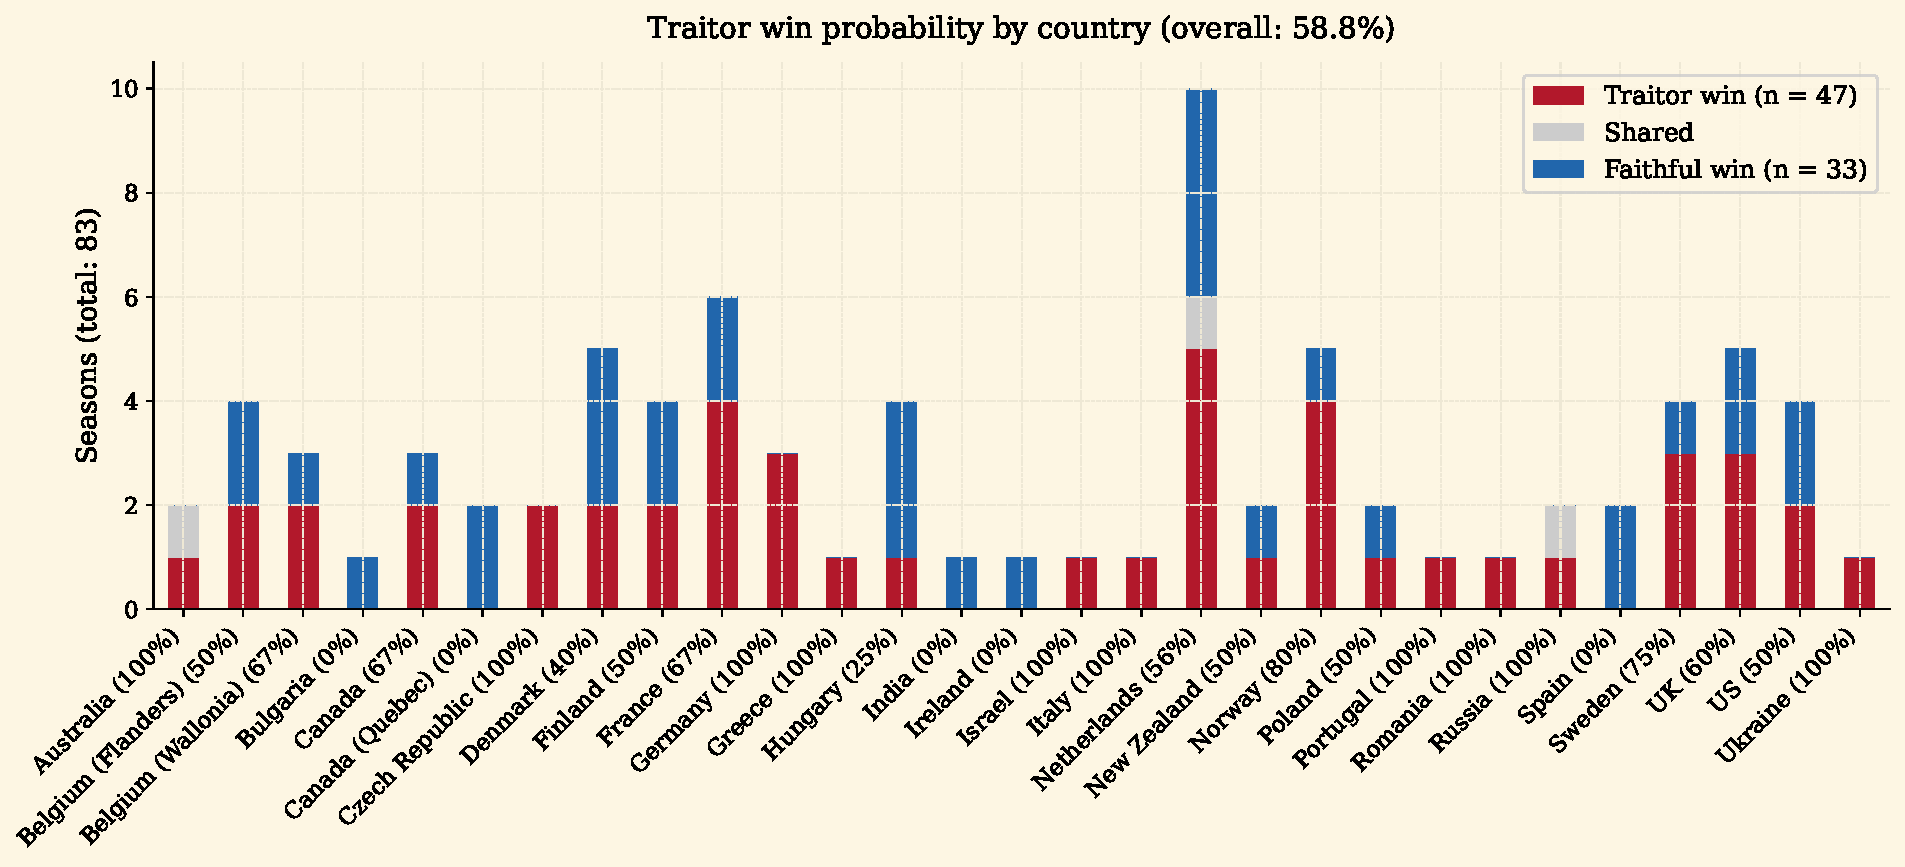
\includegraphics[width=\textwidth]{fig_tv_outcomes.pdf}
        \end{center}
    \end{frame}

            \begin{frame}

                \begin{center}
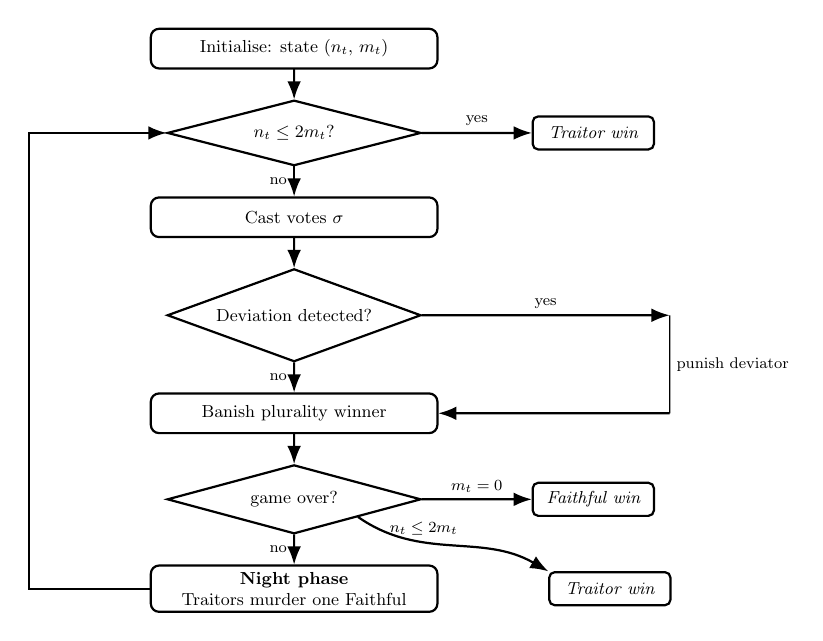
\begin{tikzpicture}[
  node distance=0.55cm,
  box/.style={
    rectangle, rounded corners=3pt, draw, thick,
    minimum width=5.2cm, minimum height=0.72cm,
    align=center, font=\small},
  dec/.style={
    diamond, draw, thick, aspect=2.5,
    minimum width=4.6cm, align=center, font=\small},
  res/.style={
    rectangle, draw, thick, rounded corners=2pt,
    minimum width=2.2cm, minimum height=0.60cm,
    align=center, font=\small\itshape},
  arr/.style={-Latex, thick},
                scale=.7,
                transform shape,
]

  % ── Main spine ──────────────────────────────────────────────────────────
  \node[box]  (init)
      {Initialise: state \((n_t,\,m_t)\)};
  \node[dec,  below=0.55cm of init]    (wpre)
      {\(n_t \leq 2m_t\)?};
  \node[box,  below=0.55cm of wpre]    (votes)
      {Cast votes \(\sigma\)};
  \node[dec,  below=0.55cm of votes]   (detect)
      {Deviation detected?};
  \node[box,  below=0.55cm of detect]  (banish)
      {Banish plurality winner};
  \node[dec,  below=0.55cm of banish]  (wpost)
      {game over?};
  \node[box,  below=0.55cm of wpost]   (night)
      {\textbf{Night phase}\\
       Traitors murder one Faithful};

  % ── Terminal outcome nodes ───────────────────────────────────────────────
  \node[res, right=2.0cm of wpre]   (Tw1) {Traitor win};
  \node[res, right=2.0cm of wpost]  (Fw)  {Faithful win};
  \node[res, right=2.0cm of night]  (Tw2) {Traitor win};

  % ── Spine arrows ────────────────────────────────────────────────────────
  \draw[arr] (init)   -- (wpre);
  \draw[arr] (wpre)   -- node[left,  font=\footnotesize]{no}  (votes);
  \draw[arr] (votes)  -- (detect);
  \draw[arr] (detect) -- node[left,  font=\footnotesize]{no}  (banish);
  \draw[arr] (banish) -- (wpost);
  \draw[arr] (wpost)  -- node[left,  font=\footnotesize]{no}  (night);

  % ── Win condition exits ──────────────────────────────────────────────────
  \draw[arr] (wpre.east) --
      node[above, font=\footnotesize]{yes} (Tw1.west);
  \draw[arr] (wpost.east) --
      node[above, font=\footnotesize]{\(m_t = 0\)} (Fw.west);
  % Tw2 sits beside night, so the arrow curves well clear of the night box.
  \draw[arr] (wpost.south east) to[out=-35, in=150]
      node[above, font=\footnotesize, pos=0.35]{\(n_t \leq 2m_t\)}
      (Tw2.north west);

  % ── Deviation bypass: detect →yes→ right → down → into banish.east ──────
  % byp1: directly to the right of detect, past all right-side res nodes.
  % byp2: same x as byp1, at banish centre height.
  % The final segment goes leftward into banish.east (arrowhead there).
  \coordinate (byp1) at ($(detect.east) + (4.5cm, 0)$);
  \coordinate (byp2) at (byp1 |- banish);
  \draw[arr] (detect.east) --
      node[above, font=\footnotesize]{yes} (byp1);
  \draw      (byp1) --
      node[right, font=\footnotesize]{punish deviator} (byp2);
  \draw[arr] (byp2) -- (banish.east);

  % ── Loop back ───────────────────────────────────────────────────────────
  \draw[arr] (night.west) -- ++(-2.2, 0) |- (wpre.west);

\end{tikzpicture}
                \end{center}
            \end{frame}

\begin{frame}[fragile]
    \begin{center}
        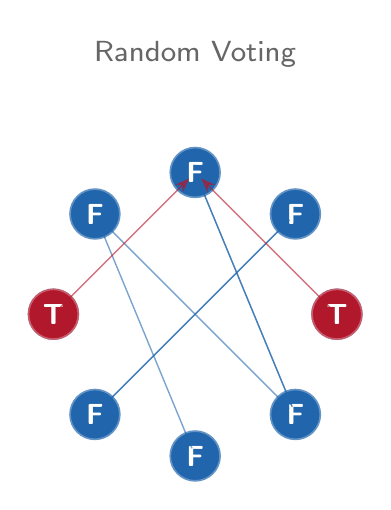
\begin{tikzpicture}[
                >=Stealth,
                font=\sffamily,
                player/.style={circle, minimum size=12pt, inner sep=0pt, line width=0.6pt,
                font=\sffamily\scriptsize\bfseries, text=white},
                fnode/.style={player, fill=faithful, draw=faithful!70},
                tnode/.style={player, fill=traitor, draw=traitor!70},
                dnode/.style={player, fill=dead, draw=dead!80, opacity=0.4,
                font=\sffamily\scriptsize\bfseries, text=black!60},
                votearrow/.style={->, line width=0.5pt, opacity=0.6},
                killarrow/.style={->, line width=1.0pt, traitor, opacity=0.8},
                panellabel/.style={font=\sffamily\footnotesize\bfseries, anchor=north west},
                caption/.style={font=\sffamily\scriptsize, text=black!60, align=center},
                scale=1.5,
                transform shape,
                ]

                % ── Layout: 2 rows x 3 cols, each panel ~4.2cm wide ──
                \def\pw{4.8}   % panel width
                \def\ph{4.2}   % panel height
                \def\gap{0.6}  % gap between panels
                \def\R{1.2}    % circle radius for players

                % Panel origins (bottom-left of each)
                \coordinate (P1) at (0, \ph+\gap);
                \coordinate (P2) at (\pw+\gap, \ph+\gap);
                \coordinate (P3) at (2*\pw+2*\gap, \ph+\gap);
                \coordinate (P4) at (0, 0);
                \coordinate (P5) at (\pw+\gap, 0);
                \coordinate (P6) at (2*\pw+2*\gap, 0);

                % ── Helper: draw 8 players in a circle ──
                % Args: center, prefix, traitor list (1-indexed)
                \newcommand{\drawplayers}[3]{
                    % #1 = center, #2 = prefix, #3 = comma-separated traitor positions
                    \foreach \i in {1,...,8} {
                        \pgfmathsetmacro{\angle}{90 - (\i-1)*45}
                        \coordinate (#2-\i) at ($(#1) + (\angle:\R)$);
                    }
                    % Draw faithful first (F label), then traitors on top (T label)
                    \foreach \i in {1,...,8} {
                        \node[fnode] at (#2-\i) {F};
                    }
                    \foreach \t in {#3} {
                        \node[tnode] at (#2-\t) {T};
                    }
                    }

                    % ── Panel D: Random Voting ──
                    \begin{scope}[shift=(P4)]
                        %\draw[draw=black!20, fill=white, rounded corners=3pt] (-0.3, -0.3) rectangle (\pw+0.3, \ph+0.3);
                        \node[caption] at (\pw/2, \ph-0.05) {Random Voting};

                        \pgfmathsetmacro{\cx}{\pw/2}
                        \pgfmathsetmacro{\cy}{\ph/2 - 0.15}
                        \coordinate (CD) at (\cx, \cy);
                        \drawplayers{CD}{d}{3,7}

                        % Random scattered votes (each to a different target)
                        \draw[votearrow, faithful, shorten >=3pt, shorten <=3pt] (d-1) -- (d-4);
                        \draw[votearrow, faithful, shorten >=3pt, shorten <=3pt] (d-2) -- (d-6);
                        \draw[votearrow, faithful, shorten >=3pt, shorten <=3pt] (d-4) -- (d-1);
                        \draw[votearrow, faithful, shorten >=3pt, shorten <=3pt] (d-5) -- (d-8);
                        \draw[votearrow, faithful, shorten >=3pt, shorten <=3pt] (d-6) -- (d-2);
                        \draw[votearrow, faithful, shorten >=3pt, shorten <=3pt] (d-8) -- (d-4);
                        % Traitors collude: both vote for player 1
                        \draw[votearrow, traitor, shorten >=3pt, shorten <=3pt] (d-3) -- (d-1);
                        \draw[votearrow, traitor, shorten >=3pt, shorten <=3pt] (d-7) -- (d-1);

                    \end{scope}


                \end{tikzpicture}
            \end{center}
            \end{frame}


            \begin{frame}

                \begin{proposition}[Migda\l{}\footfullcite{migdal2010} recurrence, adapted]\label{prop:migdal}
                    Let \(w(n,m)\) denote the Traitor win probability under mutual random play from
                    state \((n,m)\).  Then
                    \[
                        w(n,m) = \begin{cases}
                            0 & \text{if } m = 0, \\
                            1 & \text{if } n \leq 2m, \\[4pt]
                            \dfrac{n-m}{n}\,w(n-2,m) \;+\; \dfrac{m}{n}\,w(n-2,m-1) & \text{if } n > 2m.
                        \end{cases}
                    \]
                \end{proposition}
            
            \end{frame}

\begin{frame}[fragile]
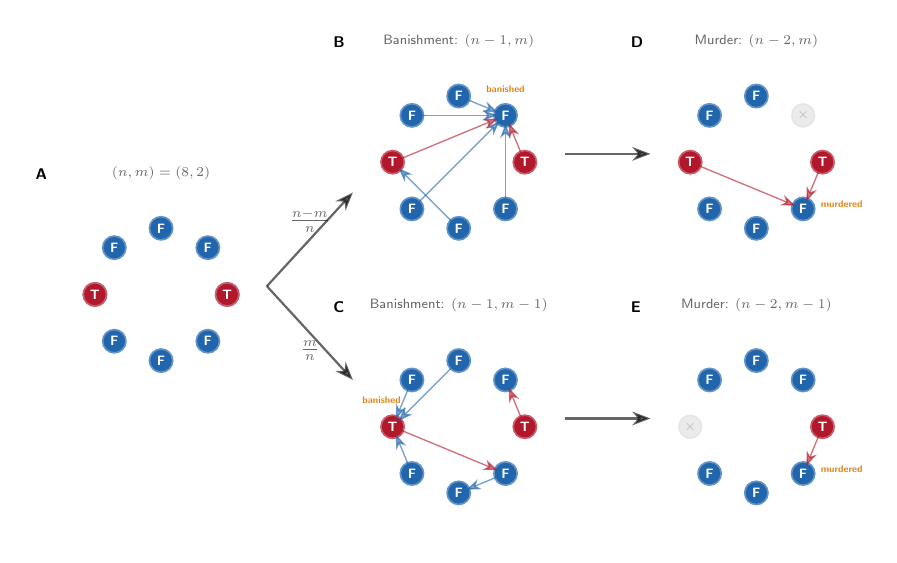
\begin{tikzpicture}[
    >=Stealth,
    font=\sffamily,
    player/.style={circle, minimum size=12pt, inner sep=0pt, line width=0.6pt,
                   font=\sffamily\scriptsize\bfseries, text=white},
    fnode/.style={player, fill=faithful, draw=faithful!70},
    tnode/.style={player, fill=traitor, draw=traitor!70},
    dnode/.style={player, fill=dead, draw=dead!80, opacity=0.4,
                  font=\sffamily\scriptsize\bfseries, text=black!60},
    votearrow/.style={->, line width=0.5pt, opacity=0.6},
    killarrow/.style={->, line width=1.0pt, traitor, opacity=0.8},
    panellabel/.style={font=\sffamily\footnotesize\bfseries, anchor=north west},
    caption/.style={font=\sffamily\scriptsize, text=black!60, align=center},
    scale=.7,
    transform shape,
]

% ── Layout: 2 rows x 3 cols, each panel ~4.2cm wide ──
\def\pw{4.8}   % panel width
\def\ph{4.2}   % panel height
\def\gap{0.6}  % gap between panels
\def\R{1.2}    % circle radius for players

% Panel origins (bottom-left of each)
\coordinate (P1) at (0, \ph-3*\gap);
\coordinate (P2) at (\pw+\gap, \ph+\gap);
\coordinate (P3) at (2*\pw+2*\gap, \ph+\gap);
\coordinate (P5) at (\pw+\gap, 0);
\coordinate (P6) at (2*\pw+2*\gap, 0);

% ── Helper: draw 8 players in a circle ──
% Args: center, prefix, traitor list (1-indexed)
\newcommand{\drawplayers}[3]{
    % #1 = center, #2 = prefix, #3 = comma-separated traitor positions
    \foreach \i in {1,...,8} {
        \pgfmathsetmacro{\angle}{90 - (\i-1)*45}
        \coordinate (#2-\i) at ($(#1) + (\angle:\R)$);
    }
    % Draw faithful first (F label), then traitors on top (T label)
    \foreach \i in {1,...,8} {
        \node[fnode] at (#2-\i) {F};
    }
    \foreach \t in {#3} {
        \node[tnode] at (#2-\t) {T};
    }
}

% ══════════════════════════════════════════════════════════════
% TOP ROW: Game phases
% ══════════════════════════════════════════════════════════════

% ── Panel A: Roles ──
\begin{scope}[shift=(P1)]
    %\draw[draw=black!20, fill=white, rounded corners=3pt] (-0.3, -0.3) rectangle (\pw+0.3, \ph+0.3);
    \node[panellabel] at (0, \ph+0.15) {A};
    \node[caption] at (\pw/2, \ph-0.05) {\((n, m)=(8, 2)\)};

    \pgfmathsetmacro{\cx}{\pw/2}
    \pgfmathsetmacro{\cy}{\ph/2 - 0.15}
    \coordinate (CA) at (\cx, \cy);
    \drawplayers{CA}{a}{3,7}

    % % Legend
    % \node[fnode, minimum size=10pt] at (3.35, 0.6) {F};
    % \node[font=\sffamily\tiny, text=faithful, anchor=west] at (3.55, 0.6) {Faithful};
    % \node[tnode, minimum size=10pt] at (3.35, 0.25) {T};
    % \node[font=\sffamily\tiny, text=traitor, anchor=west] at (3.55, 0.25) {Traitor};

\end{scope}

% ── Panel B: Night (Murder) ──
\begin{scope}[shift=(P2)]
    %\draw[draw=black!20, fill=white, rounded corners=3pt] (-0.3, -0.3) rectangle (\pw+0.3, \ph+0.3);
    \node[panellabel] at (0, \ph+0.15) {B};
    \node[caption] at (\pw/2, \ph-0.05) {Banishment: \((n - 1, m)\)};

    \pgfmathsetmacro{\cx}{\pw/2}
    \pgfmathsetmacro{\cy}{\ph/2 - 0.15}
    \coordinate (CC) at (\cx, \cy);

    \foreach \i in {1,...,8} {
        \pgfmathsetmacro{\angle}{90 - (\i-1)*45}
        \coordinate (c-\i) at ($(CC) + (\angle:\R)$);
    }
    \foreach \i in {1,2,4,5,6,8} {
        \node[fnode] at (c-\i) {F};
    }
    \node[tnode] at (c-3) {T};
    \node[tnode] at (c-7) {T};

    \foreach \src in {1,4,6,8} {
        \draw[votearrow, faithful, shorten >=3pt, shorten <=3pt] (c-\src) -- (c-2);
    }
        \draw[votearrow, faithful, shorten >=3pt, shorten <=3pt] (c-5) -- (c-7);
    \draw[votearrow, traitor, shorten >=3pt, shorten <=3pt] (c-3) -- (c-2);
    \draw[votearrow, traitor, shorten >=3pt, shorten <=3pt] (c-7) -- (c-2);

    % Banished marker
    \node[font=\sffamily\tiny\bfseries, text=warn, anchor=south] at ($(c-2)+(0, 0.3)$) {banished};
\end{scope}

% ── Panel C: Day (Banishment) ──
\begin{scope}[shift=(P3)]
    %\draw[draw=black!20, fill=white, rounded corners=3pt] (-0.3, -0.3) rectangle (\pw+0.3, \ph+0.3);
    \node[panellabel] at (0, \ph+0.15) {D};
    \node[caption] at (\pw/2, \ph-0.05) {Murder: \((n - 2, m)\)};

    \pgfmathsetmacro{\cx}{\pw/2}
    \pgfmathsetmacro{\cy}{\ph/2 - 0.15}
    \coordinate (CC) at (\cx, \cy);

    \foreach \i in {1,...,8} {
        \pgfmathsetmacro{\angle}{90 - (\i-1)*45}
        \coordinate (c-\i) at ($(CC) + (\angle:\R)$);
    }
    \foreach \i in {1,4,5,6,8} {
        \node[fnode] at (c-\i) {F};
    }
    \node[tnode] at (c-3) {T};
    \node[tnode] at (c-7) {T};
    \node[dnode] at (c-2) {$\times$};

    % Show some votes converging on player 2 (banished)
    \draw[votearrow, traitor, shorten >=3pt, shorten <=3pt] (c-3) -- (c-4);
    \draw[votearrow, traitor, shorten >=3pt, shorten <=3pt] (c-7) -- (c-4);

    % Banished marker
    \node[font=\sffamily\tiny\bfseries, text=warn, anchor=south] at ($(c-4)+(.7, -.1)$) {murdered};
\end{scope}

\begin{scope}[shift=(P5)]
    %\draw[draw=black!20, fill=white, rounded corners=3pt] (-0.3, -0.3) rectangle (\pw+0.3, \ph+0.3);
    \node[panellabel] at (0, \ph+0.15) {C};
    \node[caption] at (\pw/2, \ph-0.05) {Banishment: \((n - 1, m - 1)\)};

    \pgfmathsetmacro{\cx}{\pw/2}
    \pgfmathsetmacro{\cy}{\ph/2 - 0.15}
    \coordinate (CC) at (\cx, \cy);

    \foreach \i in {1,...,8} {
        \pgfmathsetmacro{\angle}{90 - (\i-1)*45}
        \coordinate (c-\i) at ($(CC) + (\angle:\R)$);
    }
    \foreach \i in {1,2,4,5,6,8} {
        \node[fnode] at (c-\i) {F};
    }
    \node[tnode] at (c-3) {T};
    \node[tnode] at (c-7) {T};

    % Show some votes converging on player 2 (banished)
    \foreach \src in {1,6,8} {
        \draw[votearrow, faithful, shorten >=3pt, shorten <=3pt] (c-\src) --
        (c-7);
    }
    \draw[votearrow, faithful, shorten >=3pt, shorten <=3pt] (c-4) -- (c-5);
    \draw[votearrow, traitor, shorten >=3pt, shorten <=3pt] (c-3) -- (c-2);
    \draw[votearrow, traitor, shorten >=3pt, shorten <=3pt] (c-7) -- (c-4);

    % Banished marker
    \node[font=\sffamily\tiny\bfseries, text=warn, anchor=south] at ($(c-7)+(-.2, 0.3)$) {banished};
\end{scope}

\begin{scope}[shift=(P6)]
    %\draw[draw=black!20, fill=white, rounded corners=3pt] (-0.3, -0.3) rectangle (\pw+0.3, \ph+0.3);
    \node[panellabel] at (0, \ph+0.15) {E};
    \node[caption] at (\pw/2, \ph-0.05) {Murder: \((n - 2, m - 1)\)};

    \pgfmathsetmacro{\cx}{\pw/2}
    \pgfmathsetmacro{\cy}{\ph/2 - 0.15}
    \coordinate (CC) at (\cx, \cy);

    \foreach \i in {1,...,8} {
        \pgfmathsetmacro{\angle}{90 - (\i-1)*45}
        \coordinate (c-\i) at ($(CC) + (\angle:\R)$);
    }
    \foreach \i in {1,2,4,5,6,8} {
        \node[fnode] at (c-\i) {F};
    }
    \node[tnode] at (c-3) {T};
    \node[dnode] at (c-7) {$\times$};

    % Show some votes converging on player 2 (banished)
    \draw[votearrow, traitor, shorten >=3pt, shorten <=3pt] (c-3) -- (c-4);

    % Banished marker
    \node[font=\sffamily\tiny\bfseries, text=warn, anchor=south] at ($(c-4)+(.7, -.1)$) {murdered};
\end{scope}

\draw[->, line width=0.8pt, opacity=0.6] (P1) + (\pw*.9, \ph/2) -- ($(P2) + (\pw/10, \ph/3)$)
    node[midway, above] {\(\frac{n - m}{n}\)};
\draw[->, line width=0.8pt, opacity=0.6] (P1) + (\pw*.9, \ph/2) -- ($(P5) + (\pw/10, 2*\ph/3)$)
    node[midway, below] {\(\frac{m}{n}\)};
\draw[->, line width=0.8pt, opacity=0.6] (P2) + (\pw*.9, \ph/2) -- ($(P3) + (\pw/10, \ph/2)$)
    node[midway, below] {};
\draw[->, line width=0.8pt, opacity=0.6] (P5) + (\pw*.9, \ph/2) -- ($(P6) + (\pw/10, \ph/2)$)
    node[midway, below] {};

\end{tikzpicture}
            \end{frame}

\begin{frame}
    \begin{center}
        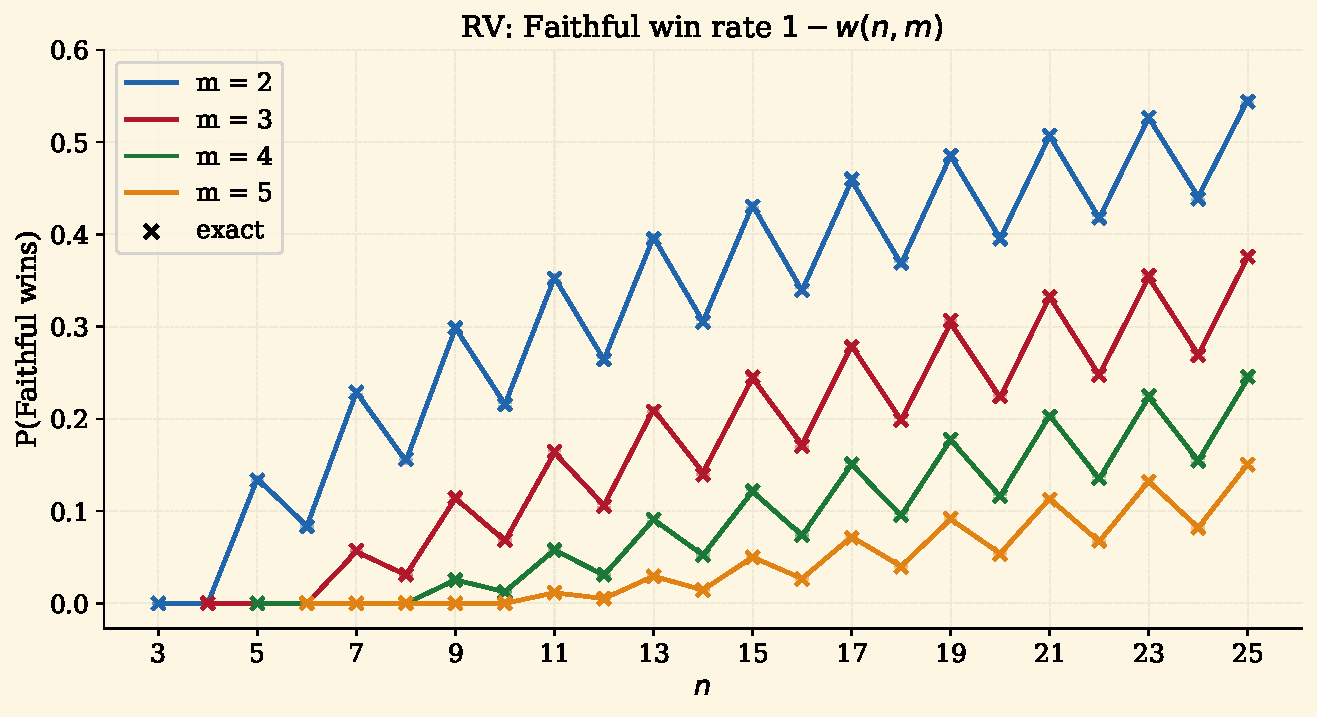
\includegraphics[width=\textwidth]{fig_w_rv.pdf}
    \end{center}
\end{frame}

\begin{frame}[fragile]

    \begin{center}
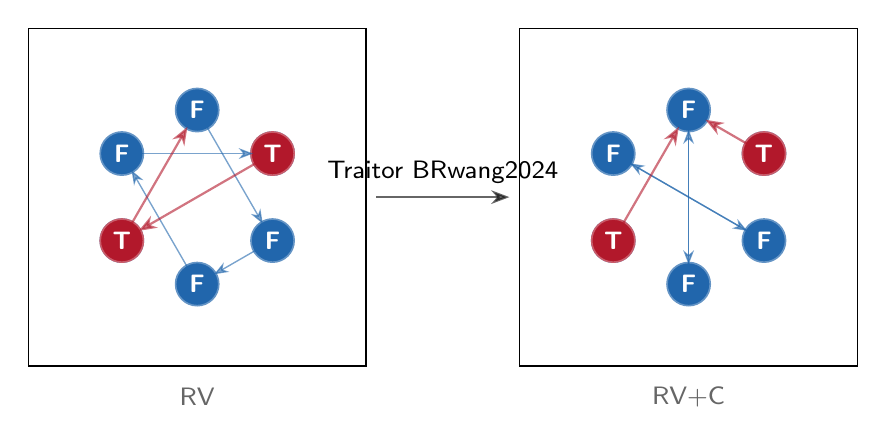
\begin{tikzpicture}[
    >=Stealth,
    font=\sffamily,
    player/.style={circle, minimum size=12pt, inner sep=0pt, line width=0.6pt,
                   font=\sffamily\scriptsize\bfseries, text=white},
    fnode/.style={player, fill=faithful, draw=faithful!70},
    tnode/.style={player, fill=traitor, draw=traitor!70},
    votearrow/.style={->, line width=0.5pt, opacity=0.6,
                      shorten >=7pt, shorten <=7pt},
    caption/.style={font=\sffamily\scriptsize, text=black!60, align=center},
    panelbg/.style={},
    scale=1.3,
    transform shape,
]

\def\pw{2.8}    % panel width
\def\ph{5.4}    % vertical spacing between rows (room for down-arrow + label)
\def\R{0.85}    % circle radius for players
\def\xgap{2.0}  % horizontal gap between panels (room for arrows + labels)

% First row panels: 3 panels left-aligned
\coordinate (P1) at (0, \ph);
\coordinate (P2) at (\pw+\xgap, \ph);
\coordinate (P3) at (2*\pw+2*\xgap, \ph);

% Total top-row width: 3*\pw + 2*\xgap. Bottom row spans 2*\pw + \xgap.
% Centre offset = (3*\pw + 2*\xgap - (2*\pw + \xgap)) / 2 = (\pw + \xgap)/2.
% Second row panels: centred under the top row
\coordinate (P4) at ({(\pw+\xgap)/2}, 0);
\coordinate (P5) at ({(\pw+\xgap)/2 + \pw + \xgap}, 0);

% Helper: draw 6 players in a circle
\newcommand{\drawplayerssmall}[3]{
    % #1 = center, #2 = prefix, #3 = comma-separated traitor positions
    \foreach \i in {1,...,6} {
        \pgfmathsetmacro{\angle}{90 - (\i-1)*60}
        \coordinate (#2-\i) at ($(#1) + (\angle:\R)$);
    }
    \foreach \i in {1,...,6} {
        \node[fnode] at (#2-\i) {F};
    }
    \foreach \t in {#3} {
        \node[tnode] at (#2-\t) {T};
    }
}

% ══════════════════════════════════════════════════════════════
% TOP ROW: Three strategies
% ══════════════════════════════════════════════════════════════

% ── Panel A: Random Voting (RV) ──
\begin{scope}[shift=(P1)]
    \draw[panelbg] (-0.25, -0.25) rectangle (\pw+0.25, \pw+0.25);
    \pgfmathsetmacro{\cx}{\pw/2}
    \pgfmathsetmacro{\cy}{\pw/2}
    \coordinate (CA) at (\cx, \cy);
    \drawplayerssmall{CA}{a}{2,5}

    % Random votes: every player votes for a different other player.
    % No bidirectional pairs (otherwise opposite arrows overlap as one line).
    \draw[votearrow, draw=faithful] (a-1) -- (a-3);
    \draw[votearrow, draw=faithful] (a-3) -- (a-4);
    \draw[votearrow, draw=faithful] (a-4) -- (a-6);
    \draw[votearrow, draw=faithful] (a-6) -- (a-2);
    % Traitors vote randomly too: different targets (not colluding)
    \draw[votearrow, draw=traitor, line width=0.8pt] (a-2) -- (a-5);
    \draw[votearrow, draw=traitor, line width=0.8pt] (a-5) -- (a-1);

    \node[caption] at (\pw/2, -0.55) {RV};
\end{scope}

% ── Panel B: Random Voting with Collusion (RV+C) ──
\begin{scope}[shift=(P2)]
    \draw[panelbg] (-0.25, -0.25) rectangle (\pw+0.25, \pw+0.25);

    \pgfmathsetmacro{\cx}{\pw/2}
    \pgfmathsetmacro{\cy}{\pw/2}
    \coordinate (CB) at (\cx, \cy);
    \drawplayerssmall{CB}{b}{2,5}

    % Same random faithful votes
    \draw[votearrow, draw=faithful] (b-1) -- (b-4);
    \draw[votearrow, draw=faithful] (b-3) -- (b-6);
    \draw[votearrow, draw=faithful] (b-4) -- (b-1);
    \draw[votearrow, draw=faithful] (b-6) -- (b-3);
    % Both traitors converge on player 1
    \draw[votearrow, draw=traitor, line width=0.8pt] (b-2) -- (b-1);
    \draw[votearrow, draw=traitor, line width=0.8pt] (b-5) -- (b-1);

    \node[caption] at (\pw/2, -0.55) {RV+C};
\end{scope}

\draw[->, line width=0.8pt, opacity=0.6]
    ($(P1) + (\pw+0.35, \pw/2)$) -- ($(P2) + (-0.35, \pw/2)$)
    node[midway, above, font=\sffamily\scriptsize, opacity=1]
        {Traitor BR\footfullcite{wang2024}};

\end{tikzpicture}
\end{center}
\end{frame}



\begin{frame}[fragile]
    \begin{center}
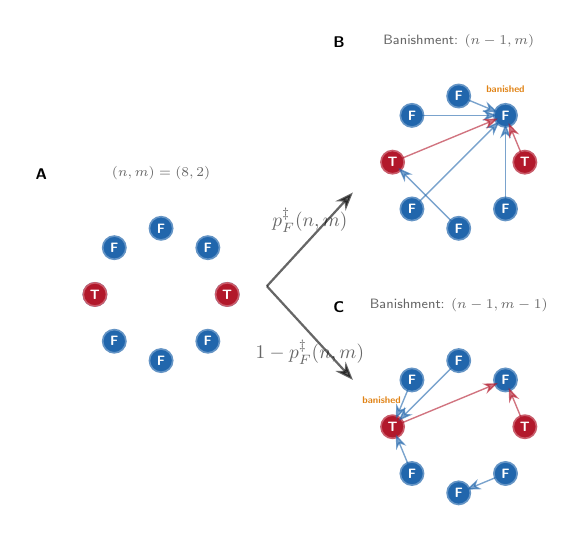
\begin{tikzpicture}[
    >=Stealth,
    font=\sffamily,
    player/.style={circle, minimum size=12pt, inner sep=0pt, line width=0.6pt,
                   font=\sffamily\scriptsize\bfseries, text=white},
    fnode/.style={player, fill=faithful, draw=faithful!70},
    tnode/.style={player, fill=traitor, draw=traitor!70},
    dnode/.style={player, fill=dead, draw=dead!80, opacity=0.4,
                  font=\sffamily\scriptsize\bfseries, text=black!60},
    votearrow/.style={->, line width=0.5pt, opacity=0.6},
    killarrow/.style={->, line width=1.0pt, traitor, opacity=0.8},
    panellabel/.style={font=\sffamily\footnotesize\bfseries, anchor=north west},
    caption/.style={font=\sffamily\scriptsize, text=black!60, align=center},
    scale=.7,
    transform shape,
]

% ── Layout: 2 rows x 3 cols, each panel ~4.2cm wide ──
\def\pw{4.8}   % panel width
\def\ph{4.2}   % panel height
\def\gap{0.6}  % gap between panels
\def\R{1.2}    % circle radius for players

% Panel origins (bottom-left of each)
\coordinate (P1) at (0, \ph-3*\gap);
\coordinate (P2) at (\pw+\gap, \ph+\gap);
\coordinate (P3) at (2*\pw+2*\gap, \ph+\gap);
\coordinate (P5) at (\pw+\gap, 0);
\coordinate (P6) at (2*\pw+2*\gap, 0);

% ── Helper: draw 8 players in a circle ──
% Args: center, prefix, traitor list (1-indexed)
\newcommand{\drawplayers}[3]{
    % #1 = center, #2 = prefix, #3 = comma-separated traitor positions
    \foreach \i in {1,...,8} {
        \pgfmathsetmacro{\angle}{90 - (\i-1)*45}
        \coordinate (#2-\i) at ($(#1) + (\angle:\R)$);
    }
    % Draw faithful first (F label), then traitors on top (T label)
    \foreach \i in {1,...,8} {
        \node[fnode] at (#2-\i) {F};
    }
    \foreach \t in {#3} {
        \node[tnode] at (#2-\t) {T};
    }
}

% ══════════════════════════════════════════════════════════════
% TOP ROW: Game phases
% ══════════════════════════════════════════════════════════════

% ── Panel A: Roles ──
\begin{scope}[shift=(P1)]
    %\draw[draw=black!20, fill=white, rounded corners=3pt] (-0.3, -0.3) rectangle (\pw+0.3, \ph+0.3);
    \node[panellabel] at (0, \ph+0.15) {A};
    \node[caption] at (\pw/2, \ph-0.05) {\((n, m)=(8, 2)\)};

    \pgfmathsetmacro{\cx}{\pw/2}
    \pgfmathsetmacro{\cy}{\ph/2 - 0.15}
    \coordinate (CA) at (\cx, \cy);
    \drawplayers{CA}{a}{3,7}

    % % Legend
    % \node[fnode, minimum size=10pt] at (3.35, 0.6) {F};
    % \node[font=\sffamily\tiny, text=faithful, anchor=west] at (3.55, 0.6) {Faithful};
    % \node[tnode, minimum size=10pt] at (3.35, 0.25) {T};
    % \node[font=\sffamily\tiny, text=traitor, anchor=west] at (3.55, 0.25) {Traitor};

\end{scope}

% ── Panel B: Night (Murder) ──
\begin{scope}[shift=(P2)]
    %\draw[draw=black!20, fill=white, rounded corners=3pt] (-0.3, -0.3) rectangle (\pw+0.3, \ph+0.3);
    \node[panellabel] at (0, \ph+0.15) {B};
    \node[caption] at (\pw/2, \ph-0.05) {Banishment: \((n - 1, m)\)};

    \pgfmathsetmacro{\cx}{\pw/2}
    \pgfmathsetmacro{\cy}{\ph/2 - 0.15}
    \coordinate (CC) at (\cx, \cy);

    \foreach \i in {1,...,8} {
        \pgfmathsetmacro{\angle}{90 - (\i-1)*45}
        \coordinate (c-\i) at ($(CC) + (\angle:\R)$);
    }
    \foreach \i in {1,2,4,5,6,8} {
        \node[fnode] at (c-\i) {F};
    }
    \node[tnode] at (c-3) {T};
    \node[tnode] at (c-7) {T};

    \foreach \src in {1,4,6,8} {
        \draw[votearrow, faithful, shorten >=3pt, shorten <=3pt] (c-\src) -- (c-2);
    }
        \draw[votearrow, faithful, shorten >=3pt, shorten <=3pt] (c-5) -- (c-7);
    \draw[votearrow, traitor, shorten >=3pt, shorten <=3pt] (c-3) -- (c-2);
    \draw[votearrow, traitor, shorten >=3pt, shorten <=3pt] (c-7) -- (c-2);

    % Banished marker
    \node[font=\sffamily\tiny\bfseries, text=warn, anchor=south] at ($(c-2)+(0, 0.3)$) {banished};
\end{scope}


\begin{scope}[shift=(P5)]
    %\draw[draw=black!20, fill=white, rounded corners=3pt] (-0.3, -0.3) rectangle (\pw+0.3, \ph+0.3);
    \node[panellabel] at (0, \ph+0.15) {C};
    \node[caption] at (\pw/2, \ph-0.05) {Banishment: \((n - 1, m - 1)\)};

    \pgfmathsetmacro{\cx}{\pw/2}
    \pgfmathsetmacro{\cy}{\ph/2 - 0.15}
    \coordinate (CC) at (\cx, \cy);

    \foreach \i in {1,...,8} {
        \pgfmathsetmacro{\angle}{90 - (\i-1)*45}
        \coordinate (c-\i) at ($(CC) + (\angle:\R)$);
    }
    \foreach \i in {1,2,4,5,6,8} {
        \node[fnode] at (c-\i) {F};
    }
    \node[tnode] at (c-3) {T};
    \node[tnode] at (c-7) {T};

    % Show some votes converging on player 2 (banished)
    \foreach \src in {1,6,8} {
        \draw[votearrow, faithful, shorten >=3pt, shorten <=3pt] (c-\src) --
        (c-7);
    }
    \draw[votearrow, faithful, shorten >=3pt, shorten <=3pt] (c-4) -- (c-5);
    \draw[votearrow, traitor, shorten >=3pt, shorten <=3pt] (c-3) -- (c-2);
    \draw[votearrow, traitor, shorten >=3pt, shorten <=3pt] (c-7) -- (c-2);

    % Banished marker
    \node[font=\sffamily\tiny\bfseries, text=warn, anchor=south] at ($(c-7)+(-.2, 0.3)$) {banished};
\end{scope}

\draw[->, line width=0.8pt, opacity=0.6] (P1) + (\pw*.9, \ph/2) -- ($(P2) + (\pw/10, \ph/3)$)
    node[midway, above] {\(p_F^{\ddagger}(n,m)\)};
\draw[->, line width=0.8pt, opacity=0.6] (P1) + (\pw*.9, \ph/2) -- ($(P5) + (\pw/10, 2*\ph/3)$)
    node[midway, below] {\(1-p_F^{\ddagger}(n,m)\)};

\end{tikzpicture}
\end{center}
            \end{frame}

\begin{frame}[c]
    \begin{lemma}[Collusion banishment probability]
        The probability that the eliminated player is Faithful
        under \(\sigma^\ddagger\) is
        \[
        p_F^{\ddagger}(n,m)
        =
        \frac{1}{|\Omega|}
        \sum_{v\in\Omega}
        \frac{|W(v)\cap F|}{|W(v)|},
        \]
        where \(W(v)=\{j : C_j(v)=M(v)\}\).
    \end{lemma}
\end{frame}


\begin{frame}
    \begin{center}
        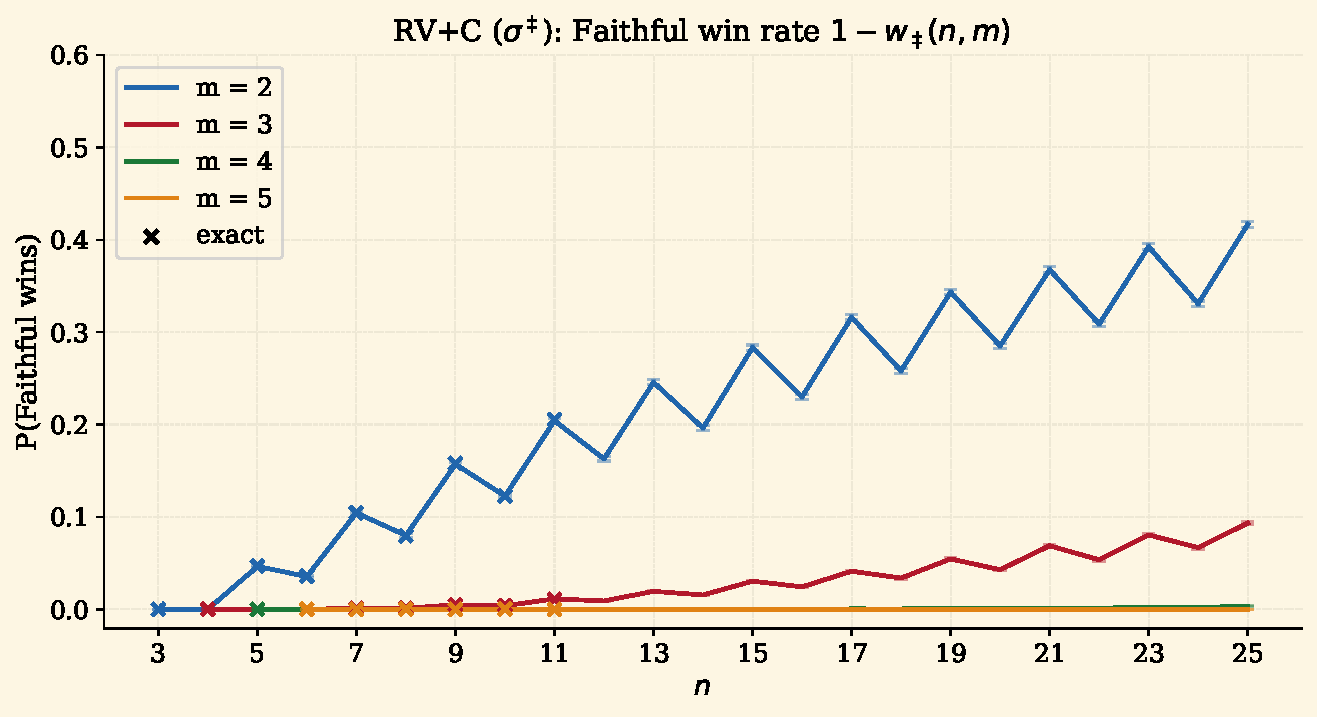
\includegraphics[width=\textwidth]{fig_w_rvc.pdf}
    \end{center}
\end{frame}

\begin{frame}[fragile]
    \begin{center}
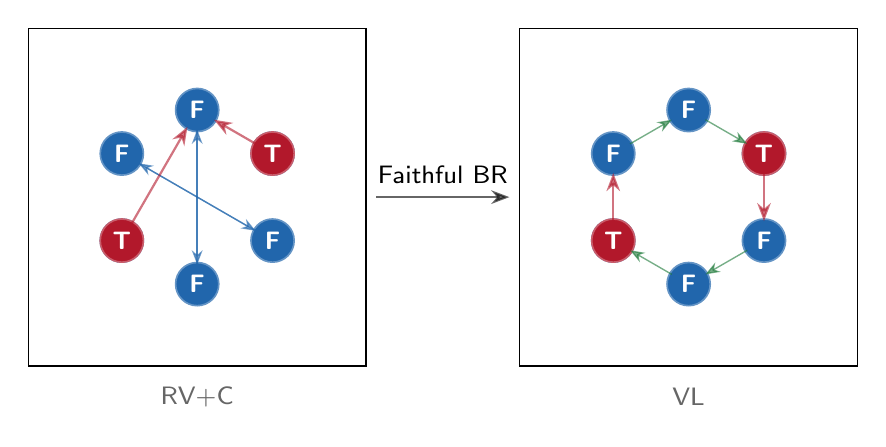
\begin{tikzpicture}[
    >=Stealth,
    font=\sffamily,
    player/.style={circle, minimum size=12pt, inner sep=0pt, line width=0.6pt,
                   font=\sffamily\scriptsize\bfseries, text=white},
    fnode/.style={player, fill=faithful, draw=faithful!70},
    tnode/.style={player, fill=traitor, draw=traitor!70},
    votearrow/.style={->, line width=0.5pt, opacity=0.6,
                      shorten >=7pt, shorten <=7pt},
    caption/.style={font=\sffamily\scriptsize, text=black!60, align=center},
    panelbg/.style={},
    scale=1.3,
    transform shape,
]

\def\pw{2.8}    % panel width
\def\ph{5.4}    % vertical spacing between rows (room for down-arrow + label)
\def\R{0.85}    % circle radius for players
\def\xgap{2.0}  % horizontal gap between panels (room for arrows + labels)

% First row panels: 3 panels left-aligned
\coordinate (P1) at (0, \ph);
\coordinate (P2) at (\pw+\xgap, \ph);
\coordinate (P3) at (2*\pw+2*\xgap, \ph);

% Total top-row width: 3*\pw + 2*\xgap. Bottom row spans 2*\pw + \xgap.
% Centre offset = (3*\pw + 2*\xgap - (2*\pw + \xgap)) / 2 = (\pw + \xgap)/2.
% Second row panels: centred under the top row
\coordinate (P4) at ({(\pw+\xgap)/2}, 0);
\coordinate (P5) at ({(\pw+\xgap)/2 + \pw + \xgap}, 0);

% Helper: draw 6 players in a circle
\newcommand{\drawplayerssmall}[3]{
    % #1 = center, #2 = prefix, #3 = comma-separated traitor positions
    \foreach \i in {1,...,6} {
        \pgfmathsetmacro{\angle}{90 - (\i-1)*60}
        \coordinate (#2-\i) at ($(#1) + (\angle:\R)$);
    }
    \foreach \i in {1,...,6} {
        \node[fnode] at (#2-\i) {F};
    }
    \foreach \t in {#3} {
        \node[tnode] at (#2-\t) {T};
    }
}

% ══════════════════════════════════════════════════════════════
% TOP ROW: Three strategies
% ══════════════════════════════════════════════════════════════

% ── Panel B: Random Voting with Collusion (RV+C) ──
\begin{scope}[shift=(P2)]
    \draw[panelbg] (-0.25, -0.25) rectangle (\pw+0.25, \pw+0.25);

    \pgfmathsetmacro{\cx}{\pw/2}
    \pgfmathsetmacro{\cy}{\pw/2}
    \coordinate (CB) at (\cx, \cy);
    \drawplayerssmall{CB}{b}{2,5}

    % Same random faithful votes
    \draw[votearrow, draw=faithful] (b-1) -- (b-4);
    \draw[votearrow, draw=faithful] (b-3) -- (b-6);
    \draw[votearrow, draw=faithful] (b-4) -- (b-1);
    \draw[votearrow, draw=faithful] (b-6) -- (b-3);
    % Both traitors converge on player 1
    \draw[votearrow, draw=traitor, line width=0.8pt] (b-2) -- (b-1);
    \draw[votearrow, draw=traitor, line width=0.8pt] (b-5) -- (b-1);

    \node[caption] at (\pw/2, -0.55) {RV+C};
\end{scope}

% ── Panel C: Vote-Left (VL) ──
\begin{scope}[shift=(P3)]
    \draw[panelbg] (-0.25, -0.25) rectangle (\pw+0.25, \pw+0.25);

    \pgfmathsetmacro{\cx}{\pw/2}
    \pgfmathsetmacro{\cy}{\pw/2}
    \coordinate (CC) at (\cx, \cy);
    \drawplayerssmall{CC}{c}{2,5}

    % Each votes for next clockwise
    \foreach \i [evaluate=\i as \j using {int(mod(\i, 6) + 1)}] in {1,...,6} {
        \pgfmathsetmacro{\isTraitor}{\i == 2 || \i == 5 ? 1 : 0}
        \ifnum\isTraitor=1
            \draw[votearrow, draw=traitor, line width=0.8pt] (c-\i) -- (c-\j);
        \else
            \draw[votearrow, draw=accent] (c-\i) -- (c-\j);
        \fi
    }

    \node[caption] at (\pw/2, -0.55) {VL};
\end{scope}

\draw[->, line width=0.8pt, opacity=0.6]
    ($(P2) + (\pw+0.35, \pw/2)$) -- ($(P3) + (-0.35, \pw/2)$)
    node[midway, above, font=\sffamily\scriptsize, opacity=1]
        {Faithful BR};


\end{tikzpicture}
    \end{center}
\end{frame}

\begin{frame}
    \begin{center}
        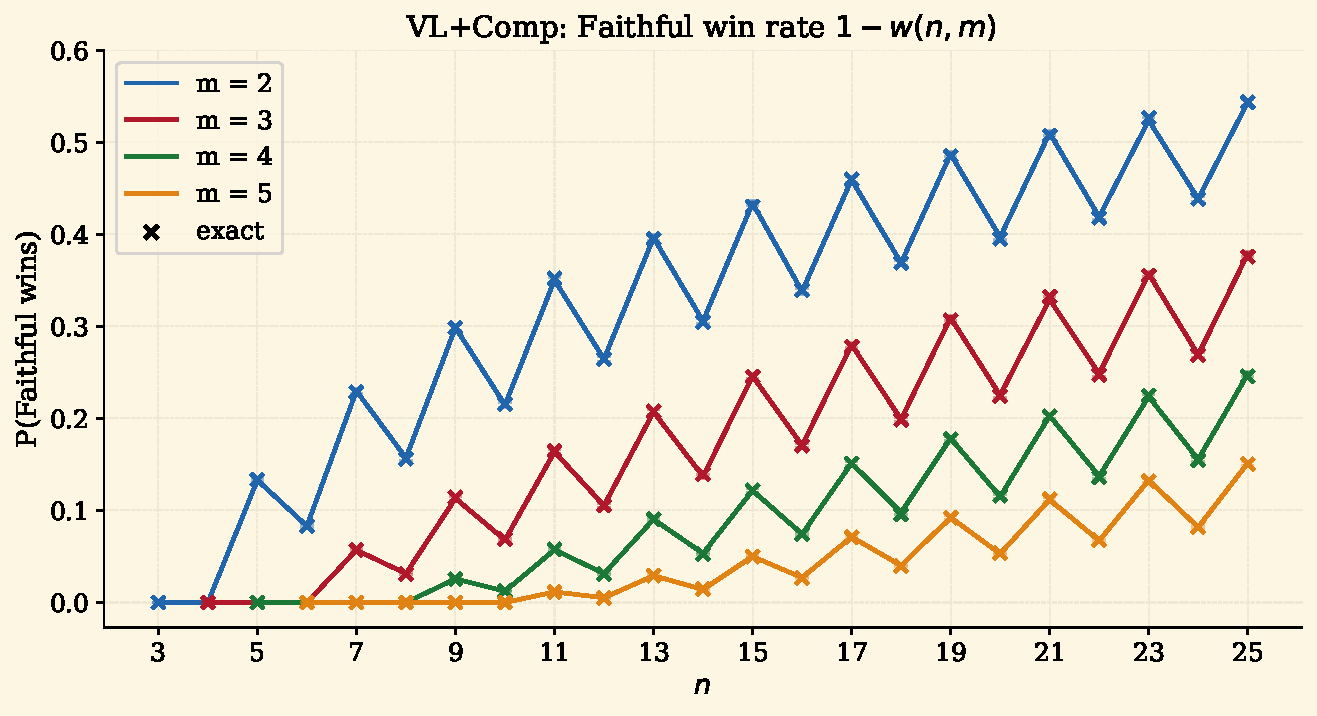
\includegraphics[width=\textwidth]{fig_w_vlcomp.pdf}
    \end{center}
\end{frame}

\begin{frame}
\begin{theorem}[Bayesian Nash Equilibrium (BNE)]\label{thm:pbe}
Vote-Left with Punishment constitutes a BNE of \(\mathrm{TG}(n, m)\) for every state with
\(n > 2m + 2\).
\end{theorem}
\end{frame}

\begin{frame}[fragile]
    \begin{center}
        \Large \(\sigma^\dagger\) (VL+Opt): the Traitors' best response
    \end{center}
    \vfill
    \begin{center}
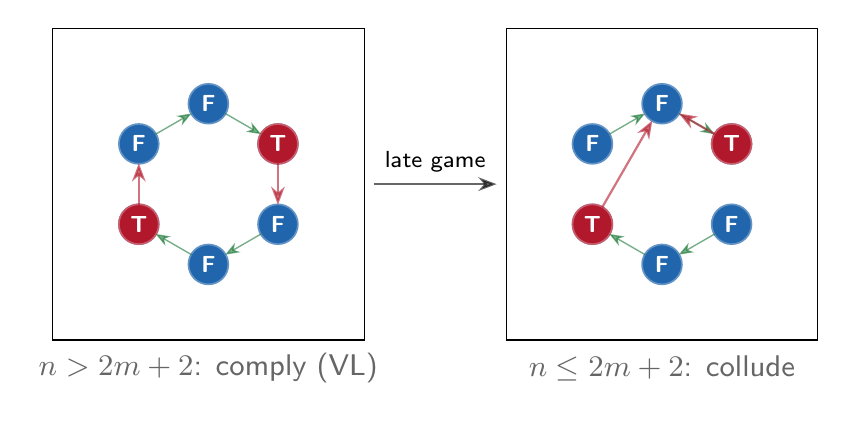
\begin{tikzpicture}[
    >=Stealth,
    font=\sffamily,
    player/.style={circle, minimum size=12pt, inner sep=0pt, line width=0.6pt,
                   font=\sffamily\scriptsize\bfseries, text=white},
    fnode/.style={player, fill=faithful, draw=faithful!70},
    tnode/.style={player, fill=traitor, draw=traitor!70},
    votearrow/.style={->, line width=0.5pt, opacity=0.6,
                      shorten >=7pt, shorten <=7pt},
    caption/.style={font=\sffamily\small, text=black!60, align=center},
    panelbg/.style={},
    scale=1.2,
    transform shape,
]

\def\pw{2.8}
\def\R{0.85}
\def\xgap{2.0}

\coordinate (PL) at (0, 0);
\coordinate (PR) at (\pw+\xgap, 0);

\newcommand{\drawplayerssmall}[3]{%
    \foreach \i in {1,...,6} {%
        \pgfmathsetmacro{\angle}{90 - (\i-1)*60}%
        \coordinate (#2-\i) at ($(#1) + (\angle:\R)$);%
    }%
    \foreach \i in {1,...,6} { \node[fnode] at (#2-\i) {F}; }%
    \foreach \t in {#3} { \node[tnode] at (#2-\t) {T}; }%
}

% ── Left panel: n > 2m+2, Traitors comply with VL ──
\begin{scope}[shift=(PL)]
    \draw[panelbg] (-0.25, -0.25) rectangle (\pw+0.25, \pw+0.25);
    \pgfmathsetmacro{\cx}{\pw/2}
    \pgfmathsetmacro{\cy}{\pw/2}
    \coordinate (CL) at (\cx, \cy);
    \drawplayerssmall{CL}{l}{2,5}

    \foreach \i [evaluate=\i as \j using {int(mod(\i, 6) + 1)}] in {1,...,6} {
        \pgfmathsetmacro{\isTraitor}{\i == 2 || \i == 5 ? 1 : 0}
        \ifnum\isTraitor=1
            \draw[votearrow, draw=traitor, line width=0.8pt] (l-\i) -- (l-\j);
        \else
            \draw[votearrow, draw=accent] (l-\i) -- (l-\j);
        \fi
    }
    \node[caption] at (\pw/2, -0.55) {\(n > 2m+2\): comply (VL)};
\end{scope}

% ── Right panel: n <= 2m+2, Traitors collude ──
\begin{scope}[shift=(PR)]
    \draw[panelbg] (-0.25, -0.25) rectangle (\pw+0.25, \pw+0.25);
    \pgfmathsetmacro{\cx}{\pw/2}
    \pgfmathsetmacro{\cy}{\pw/2}
    \coordinate (CR) at (\cx, \cy);
    \drawplayerssmall{CR}{r}{2,5}

    \foreach \i [evaluate=\i as \j using {int(mod(\i, 6) + 1)}] in {1,3,4,6} {
        \draw[votearrow, draw=accent] (r-\i) -- (r-\j);
    }
    \draw[votearrow, draw=traitor, line width=0.8pt] (r-2) -- (r-1);
    \draw[votearrow, draw=traitor, line width=0.8pt] (r-5) -- (r-1);
    \node[caption] at (\pw/2, -0.55) {\(n \leq 2m+2\): collude};
\end{scope}

\draw[->, line width=0.8pt, opacity=0.6]
    ($(PL) + (\pw+0.35, \pw/2)$) -- ($(PR) + (-0.35, \pw/2)$)
    node[midway, above, font=\sffamily\scriptsize, opacity=1] {late game};

\end{tikzpicture}
    \end{center}
\end{frame}

\begin{frame}
    \begin{proposition}[Traitor win probability under \(\sigma^\dagger\)]
        Let \(w_\dagger(n,m)\) denote the Traitor win probability under
        Vote-Left with the optimal Traitor strategy \(\sigma^\dagger\),
        starting from state \((n,m)\).  Then
        \small
        \[
        w_{\dagger}(n, m) =
        \begin{cases}
            0 & m = 0, \\[4pt]
            1 & n \leq 2m + 2, \\[4pt]
            \dfrac{n - m}{n}\, w_{\dagger}(n - 2,\, m)
             + \dfrac{m}{n}\, w_{\dagger}(n - 2,\, m - 1)
            & n > 2m + 2.
        \end{cases}
        \]
    \end{proposition}
\end{frame}

\begin{frame}
    \begin{center}
        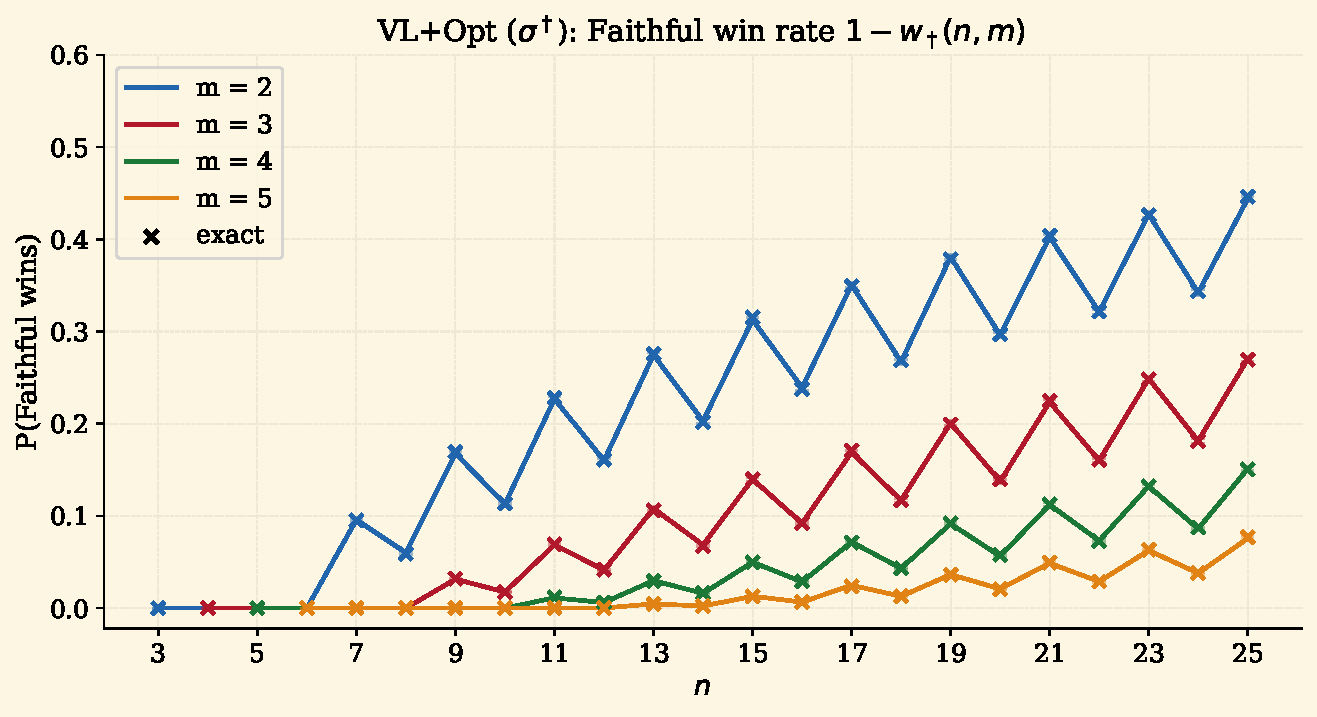
\includegraphics[width=\textwidth]{fig_w_vlopt.pdf}
    \end{center}
\end{frame}

\begin{frame}
    \begin{center}
        \resizebox{0.95\textwidth}{!}{\begin{tabular}{@{}ccccccc@{}}
\toprule
\((n, m)\) & \(w\) & RV & \(w_{\ddagger}\) & RV+C & \(w_{\dagger}\) & VL+Opt \\
\midrule
(7,\,2) & 0.771 & 0.771 & 0.896 & 0.896 & 0.905 & 0.904 \\
(8,\,2) & 0.844 & 0.846 & 0.920 & 0.920 & 0.941 & 0.940 \\
(9,\,3) & 0.886 & 0.886 & 0.995 & 0.995 & 0.968 & 0.969 \\
(10,\,3) & 0.931 & 0.932 & 0.996 & 0.996 & 0.982 & 0.983 \\
(11,\,3) & 0.835 & 0.837 & 0.989 & 0.989 & 0.931 & 0.931 \\
(11,\,5) & 0.988 & 0.989 & 1.000 & 1.000 & 1.000 & 1.000 \\
\midrule
(15,\,2) & 0.570 & 0.568 & \text{--} & 0.717 & 0.685 & 0.687 \\
(20,\,3) & 0.776 & 0.777 & \text{--} & 0.957 & 0.860 & 0.863 \\
(22,\,3) & 0.752 & 0.753 & \text{--} & 0.946 & 0.839 & 0.840 \\
(24,\,3) & 0.731 & 0.731 & \text{--} & 0.933 & 0.819 & 0.819 \\
(25,\,3) & 0.625 & 0.625 & \text{--} & 0.907 & 0.731 & 0.730 \\
(22,\,4) & 0.864 & 0.865 & \text{--} & 0.999 & 0.927 & 0.927 \\
(25,\,4) & 0.754 & 0.757 & \text{--} & 0.997 & 0.850 & 0.849 \\
\bottomrule
\end{tabular}
}
    \end{center}
\end{frame}

\begin{frame}
    \begin{center}
        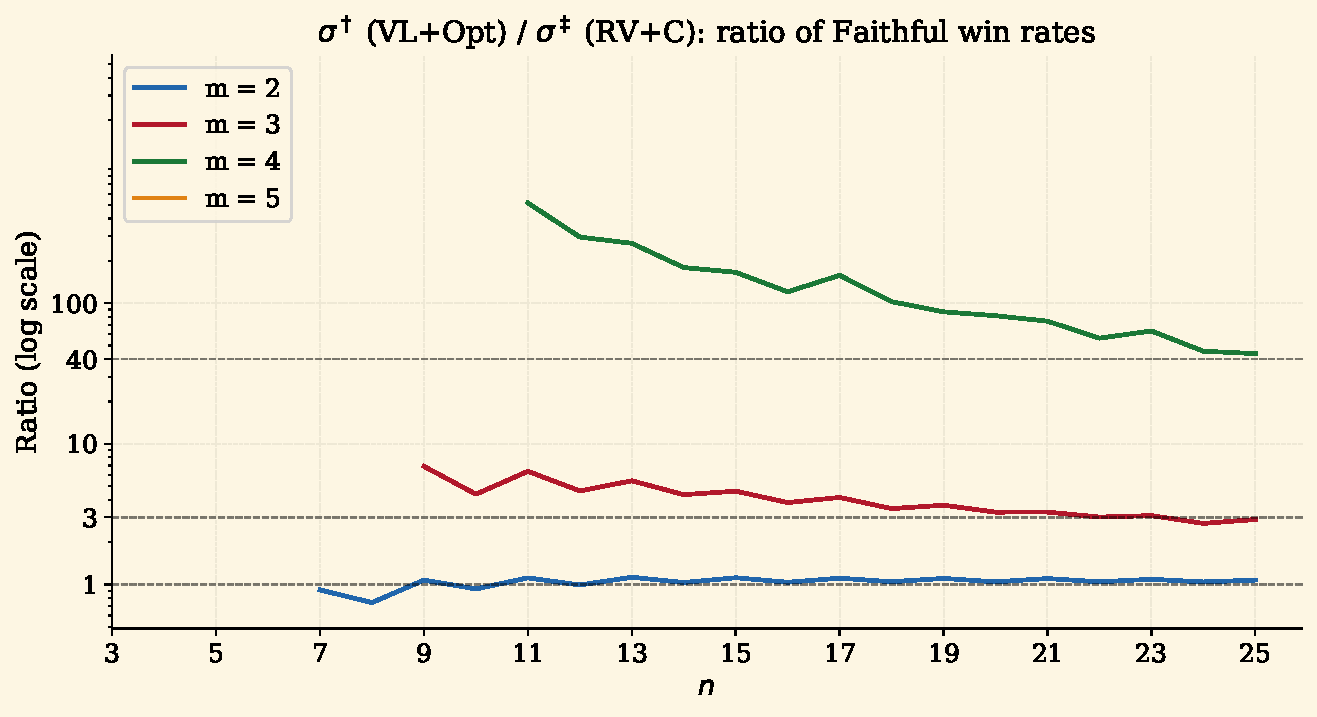
\includegraphics[width=\textwidth]{fig_ratio_vlopt_rvc.pdf}
    \end{center}
\end{frame}

\begin{frame}
    \begin{center}
        \large
        Vote-Left raises the Faithful's winning probability

        \vfill
        \LARGE
        by a factor of approximately
        \textbf{\textcolor{faithful}{three}} at \(m = 3\)

        \vfill
        by a factor of
        \textbf{\textcolor{faithful}{forty or more}} at \(m = 4\)

        \vfill
        \normalsize
        relative to random voting under Traitor collusion
    \end{center}
\end{frame}

\begin{frame}
    \begin{center}
        \Large
        The Vote-Left Equilibrium

        \vfill
        Preprint: \url{arxiv.org/abs/2605.10233}

        \vfill
        \large
        Install: \texttt{pip install backstab}\\
        Docs: \url{vknight.org/backstab}\\
        Dev: \url{github.com/drvinceknight/backstab}
    \end{center}
    \vfill
    {\footnotesize%
    \noindent\rule{\textwidth}{0.3pt}\\[4pt]%
    \hfill
    {\color{socialmastodon}vinceknight@fosstodon.org}\hfill
    {\color{socialbluesky}@vknight.bsky.social}\hfill
    {\color{sociallinkedin}/in/drvinceknight}%
    \hfill}
\end{frame}


\end{document}
